En opamp er en spennings forsterker som bl.a. kan brukes til analoge
regneoperasjoner.
\\\\
Egenskaper:
\begin{itemize}
\item Veldig høy forsterkning: $10^5$ til $10^6$.
\item Høy inngangsmotstand gjør den effektiv.
\item Stabil i forhold til temperatur.
\item Kontrollert fasegang.
\item Differansekobling på inngangen.
\end{itemize}

\begin{figure}[H]
  \caption{Symbol for en op-amp.}
  \centering
  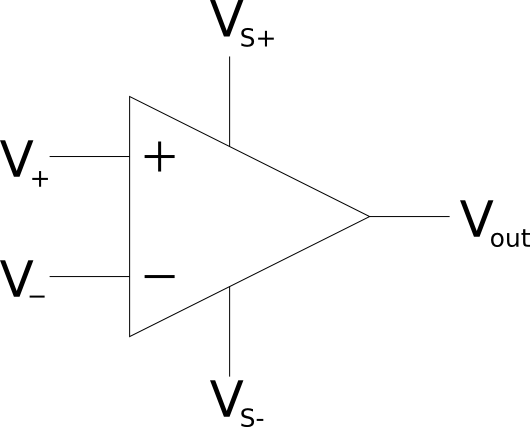
\includegraphics[width=0.5\textwidth]{./img/opamp-symbol}
\end{figure}



\paragraph{LM741} \mbox{} \\
Et eksempel på en IC implementasjon av en opamp er LM741.
\begin{figure}[H]
  \caption{LM741 pinout}
  \centering
  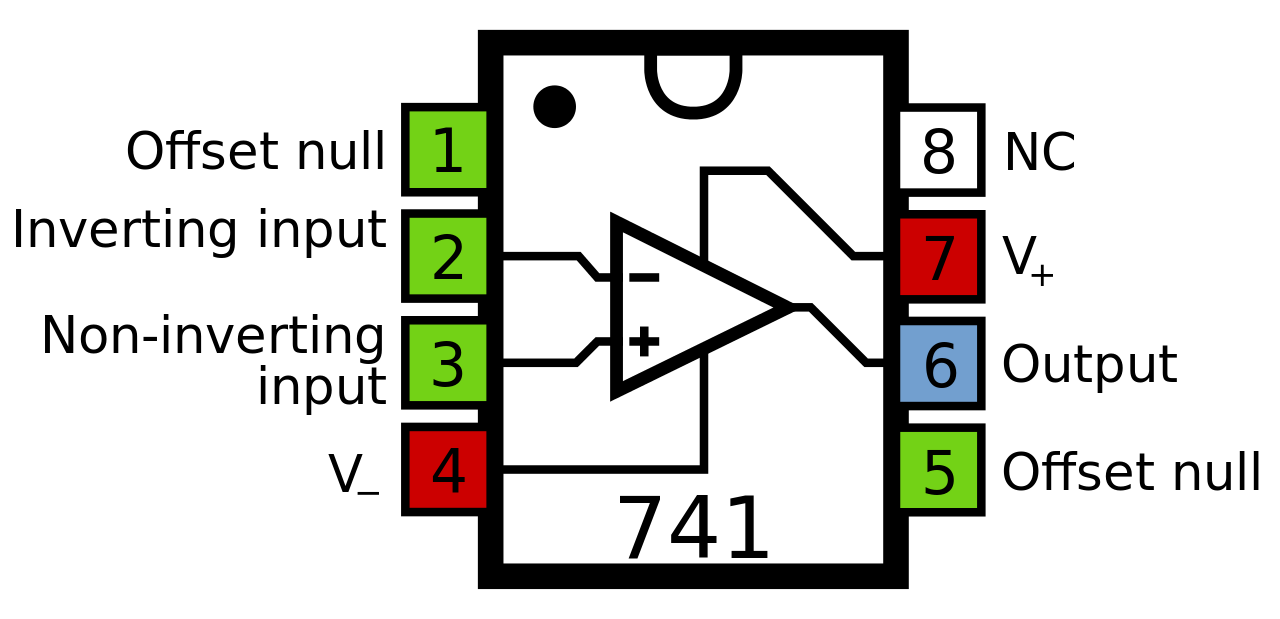
\includegraphics[width=0.5\textwidth]{./img/lm741}
\end{figure}
